Cette partie dénombre la présentation des Scénarios applicatifs de l’application.Nous allons présenter dans  ce  qui  suit,  les  imprimes écran des principales interfaces réalisées dans notre plateforme web.

\section{Page d'accueil}
\begin{figure}[H]
    \begin{center}
        \fbox{
\includegraphics[scale=0.40]{acceuil.jpg}}
        \caption{Page d'accueil}
    \end{center}
\end{figure}
La page d'accueil est la racine de laquelle l'utilisateur peut naviguer l'application.
\section{Pages Contrats}
\subsection{Liste des contrats}
\begin{figure}[H]
    \begin{center}
        \fbox{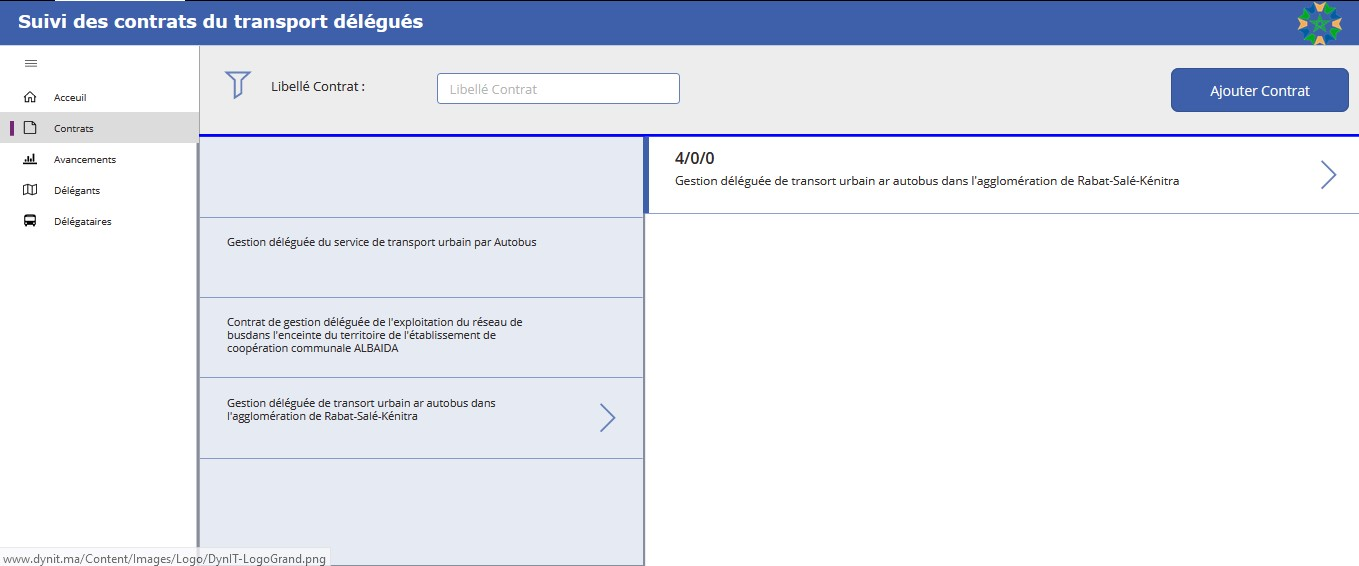
\includegraphics[scale=0.40]{contrat.jpg}}
        \caption{Liste des contrats}
    \end{center}
\end{figure}
Cette page nous affiche tous les contras et leurs avenants et révisions, comme nous pouvons trouver un contrat rapidement par son nom en le tapant dans la barre de recherche.
\subsection{Consulter Contrat}
\begin{figure}[H]
    \begin{center}
        \fbox{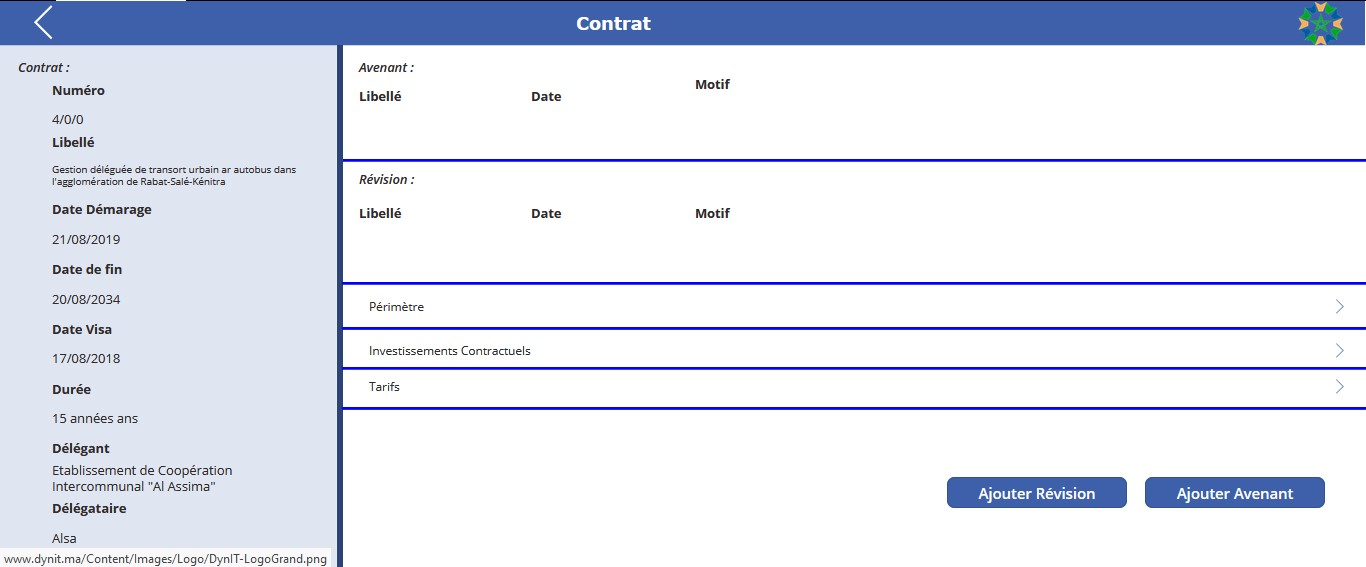
\includegraphics[scale=0.40]{aff contrat1.jpg}}
        \caption{Consulter contrat}
    \end{center}
\end{figure}
Une fois il clique sur un contrat, il est redirigé vers cette page où il trouvera toutes les informations concernant ce contrat.
\begin{figure}[H]
    \begin{center}
        \fbox{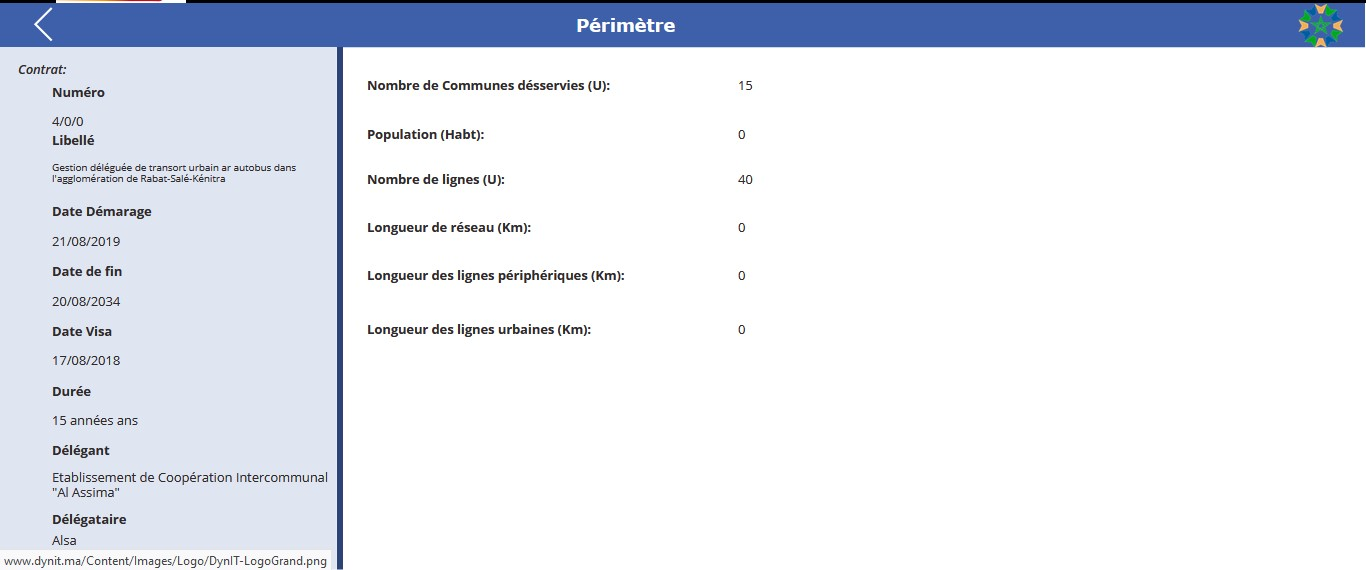
\includegraphics[scale=0.40]{affcontrat Perimetre.jpg}}
        \caption{Afficher périmètre}
    \end{center}
\end{figure}
\subsection{Ajouter Contrat}
\begin{figure}[H]
    \begin{center}
        \fbox{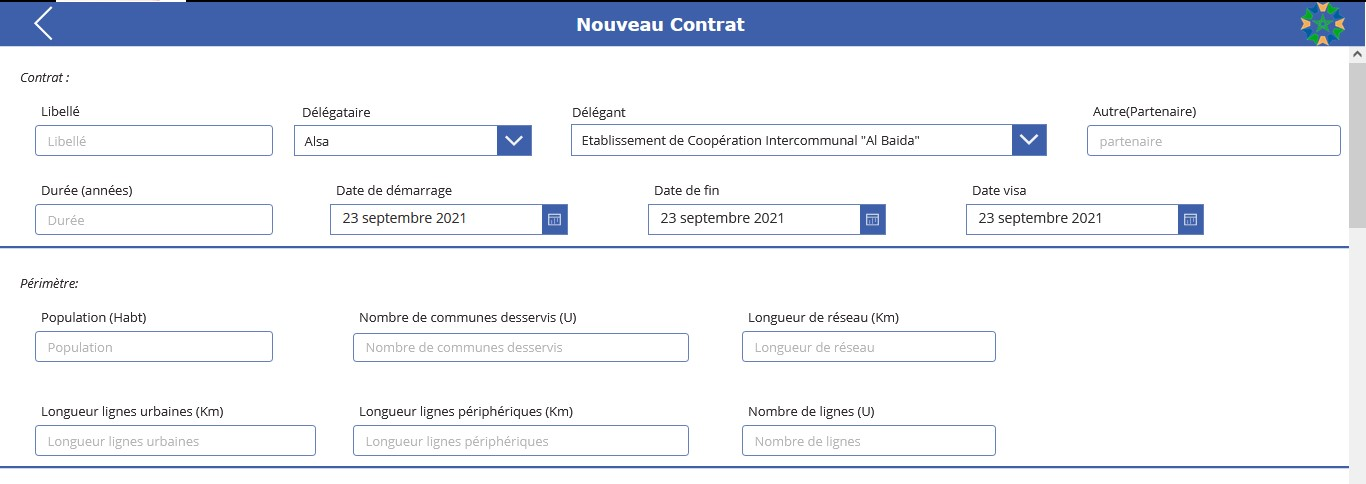
\includegraphics[scale=0.40]{Nv contrat 1.jpg}}
        \caption{Ajouter contrat}
    \end{center}
\end{figure}
\begin{figure}[H]
    \begin{center}
        \fbox{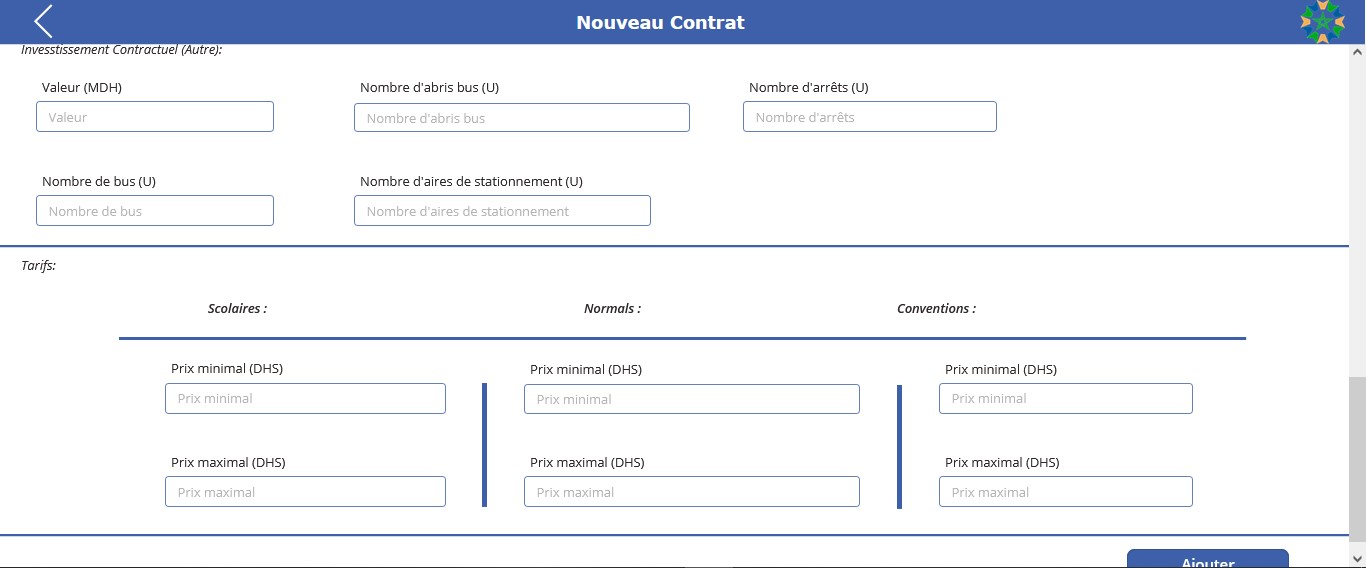
\includegraphics[scale=0.40]{Nv contrat 3.jpg}}
        \caption{Suite 1 de la figure ajouter contrat}
    \end{center}
\end{figure}
Pour ajouter un contrat, il faut renseigner les champs affichées ci-dessus.
\begin{figure}[H]
    \begin{center}
        \fbox{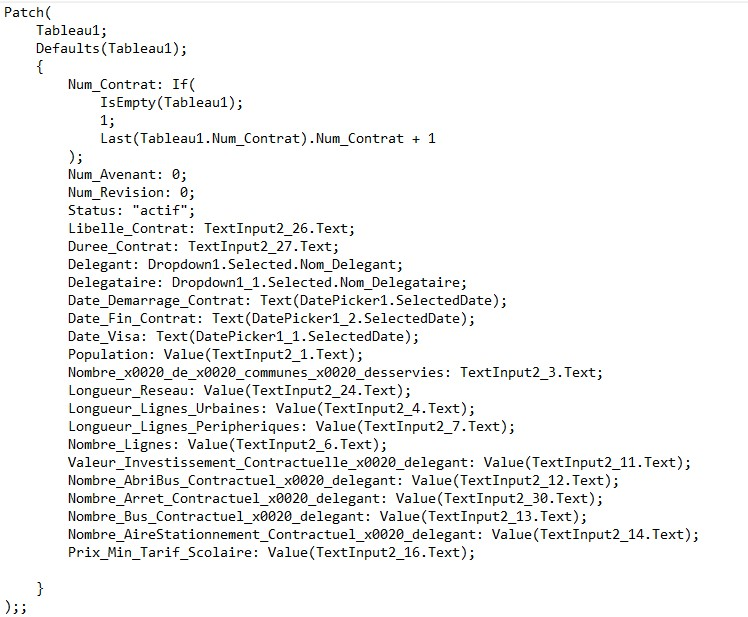
\includegraphics[scale=0.60]{patch contrat.jpg}}
        \caption{Exemple de la fonction Patch pour ajouter un contrat}
    \end{center}
\end{figure}
Après avoir rempli les champs et valider l'ajout, le contrat est ajouté à la base de données grâce à la fonction ci-dessus.
\subsection{Ajouter avenant}
\begin{figure}[H]
    \begin{center}
        \fbox{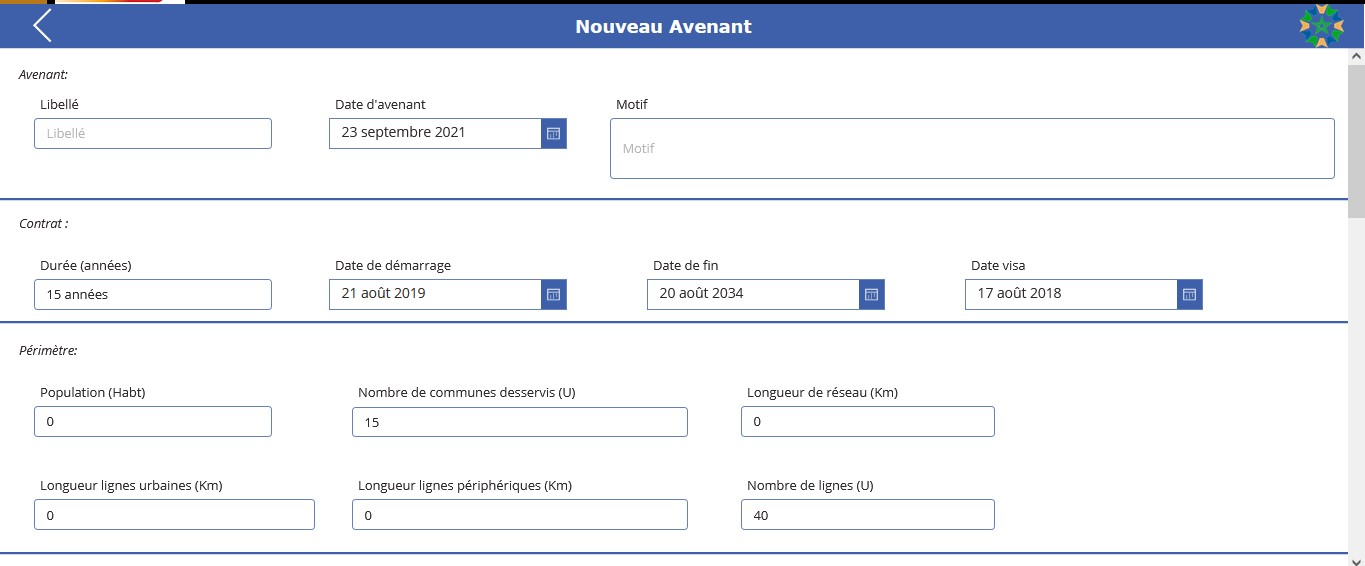
\includegraphics[scale=0.40]{Nv avenant 1.jpg}}
        \caption{Ajouter avenant}
    \end{center}
\end{figure}
Un contrat ne peut pas être modifier mais on peut générer une nouvelle version de ce dernier en ajoutant un avenant ou une révision.
\section{Pages Avancements}
\subsection{Catégories des avancements}
\begin{figure}[H]
    \begin{center}
        \fbox{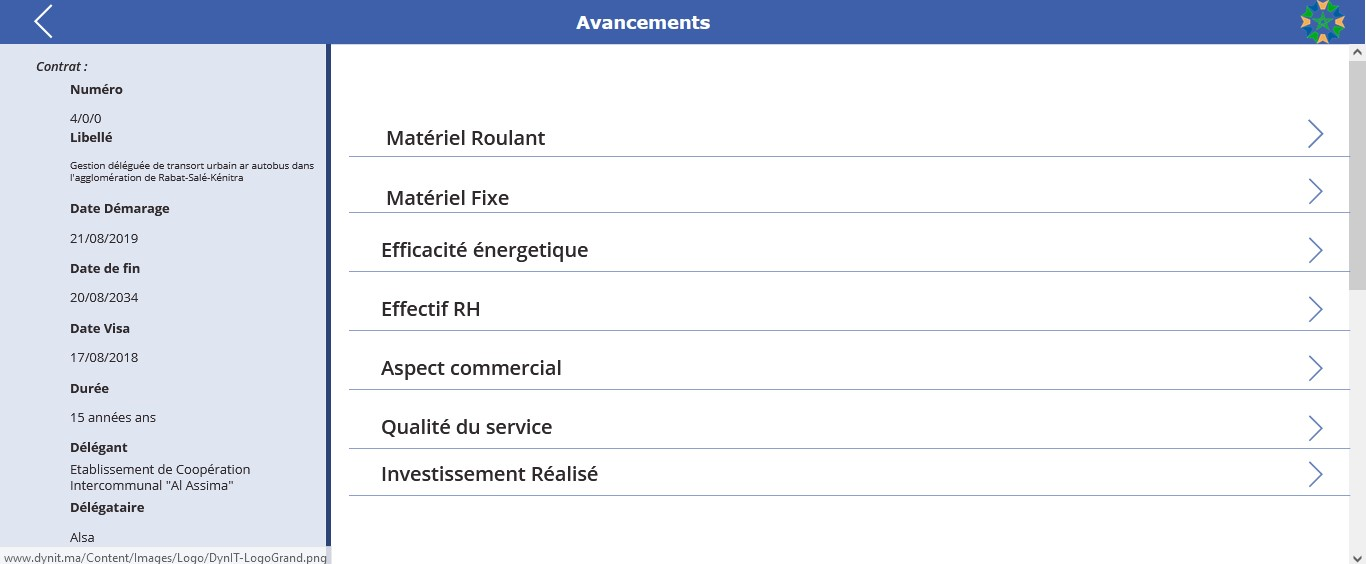
\includegraphics[scale=0.40]{Avancement2.jpg}}
        \caption{Catégories des avancements}
    \end{center}
\end{figure}
Après avoir sélectionné un contrat, une liste de catégories des avancements s'affiche.
\subsection{Afficher un avancement}
\begin{figure}[H]
    \begin{center}
        \fbox{\includegraphics[scale=0.40]{Qualité de service.jpg}}
        \caption{Afficher un avancement}
    \end{center}
\end{figure}
Après avoir choisi une catégorie -dans ce cas (Qualité de service)- une listes des avancements s'affiche selon la période sélectionnée.
\begin{figure}[H]
    \begin{center}
        \fbox{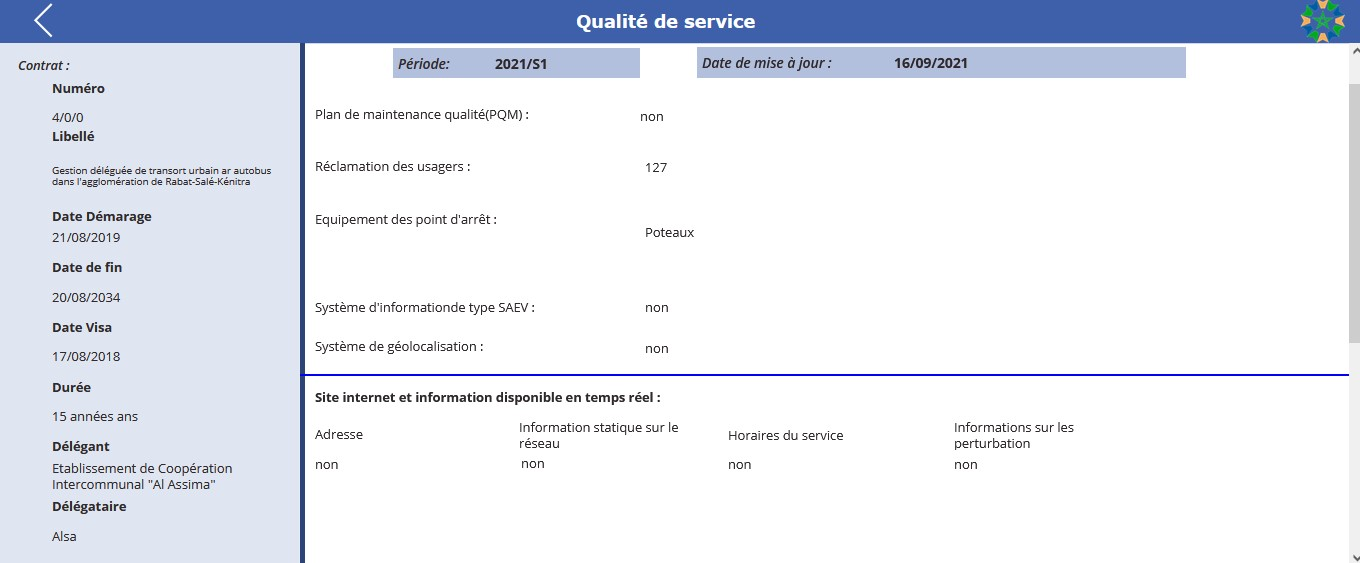
\includegraphics[scale=0.40]{aff qualite service 1.jpg}}
        \caption{Suite 1 de la figure afficher un avancement}
    \end{center}
\end{figure}
\begin{figure}[H]
    \begin{center}
        \fbox{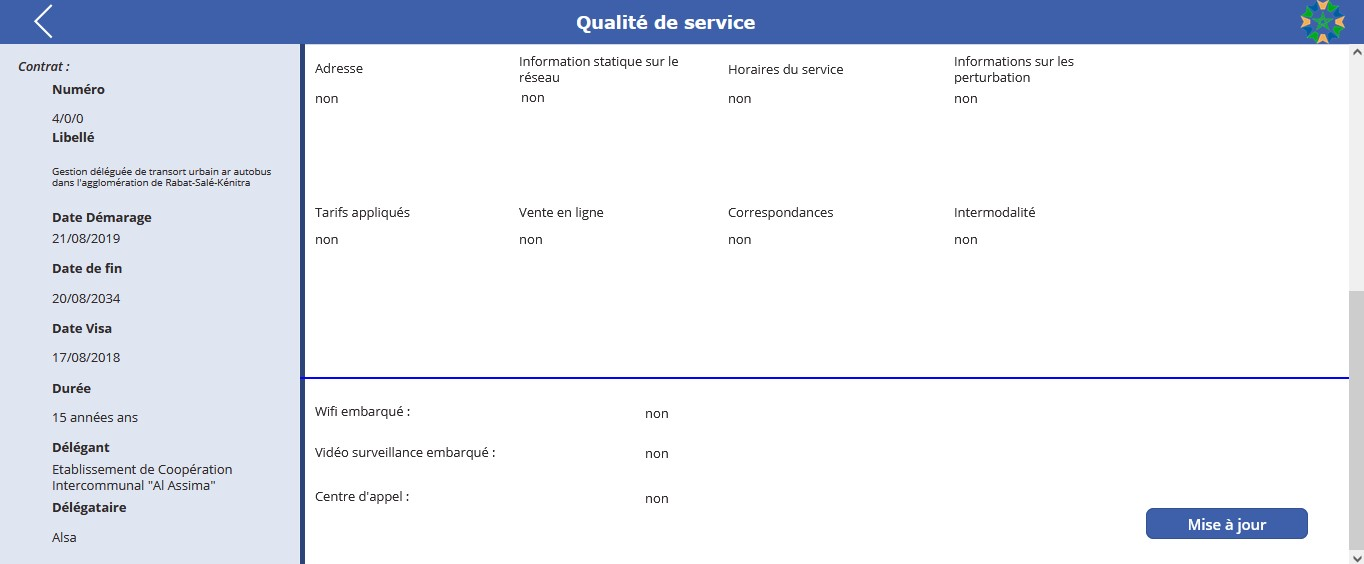
\includegraphics[scale=0.40]{aff qualite de service 2.jpg}}
        \caption{Suite 2 de la figure afficher un avancement}
    \end{center}
\end{figure}
Après avoir choisi la période voulu, l'état d'avancement s'affiche.
\subsection{Mise à jour d'avancement}
\begin{figure}[H]
    \begin{center}
        \fbox{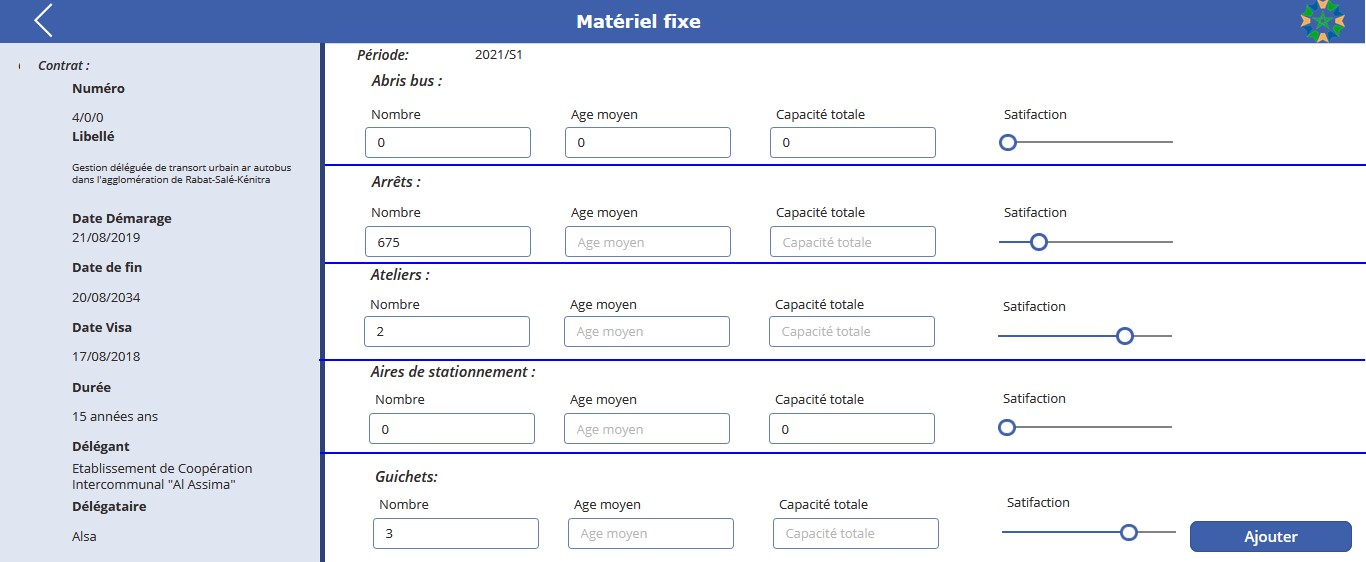
\includegraphics[scale=0.40]{mise a jour materiel fixe.jpg}}
        \caption{Mise à jour d'un avancement}
    \end{center}
\end{figure}
Pour effectuer un mise à jour d'un avancement, on clique sur le bouton 'mise à jour' puis cette page s'affiche qui contient préalablement les données déjà enregistrées, il suffit de modifier les champs voulus.
\begin{figure}[H]
    \begin{center}
        \fbox{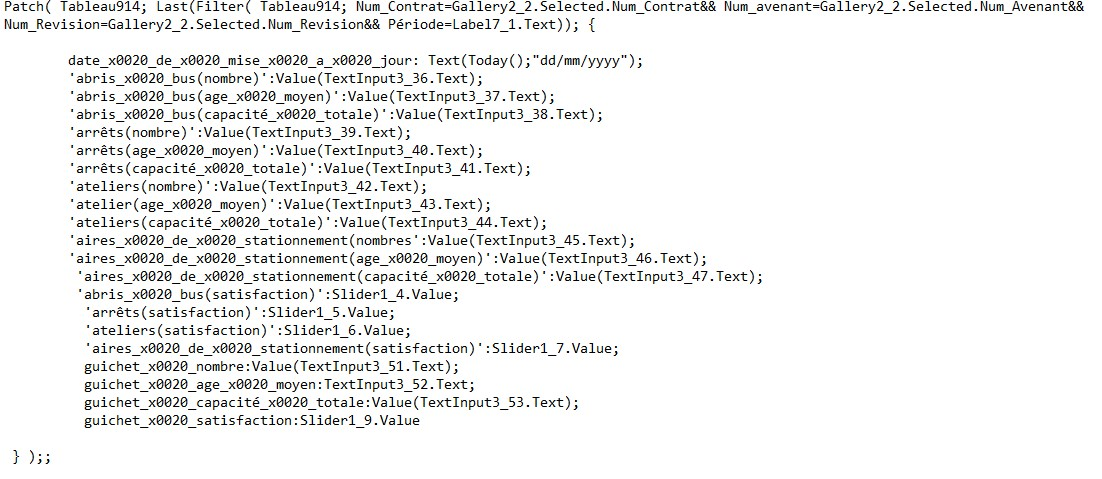
\includegraphics[scale=0.60]{patch avancement.jpg}}
        \caption{Exemple de la fonction Patch pour la mise à jour d'un avancement}
    \end{center}
\end{figure}
Après avoir modifié les champs et valider la mise à jour, l'avancement est modifié et enregistré dans la base de données grâce à la fonction ci-dessus.
\subsection{Ajouter un avancement}
\begin{figure}[H]
    \begin{center}
        \fbox{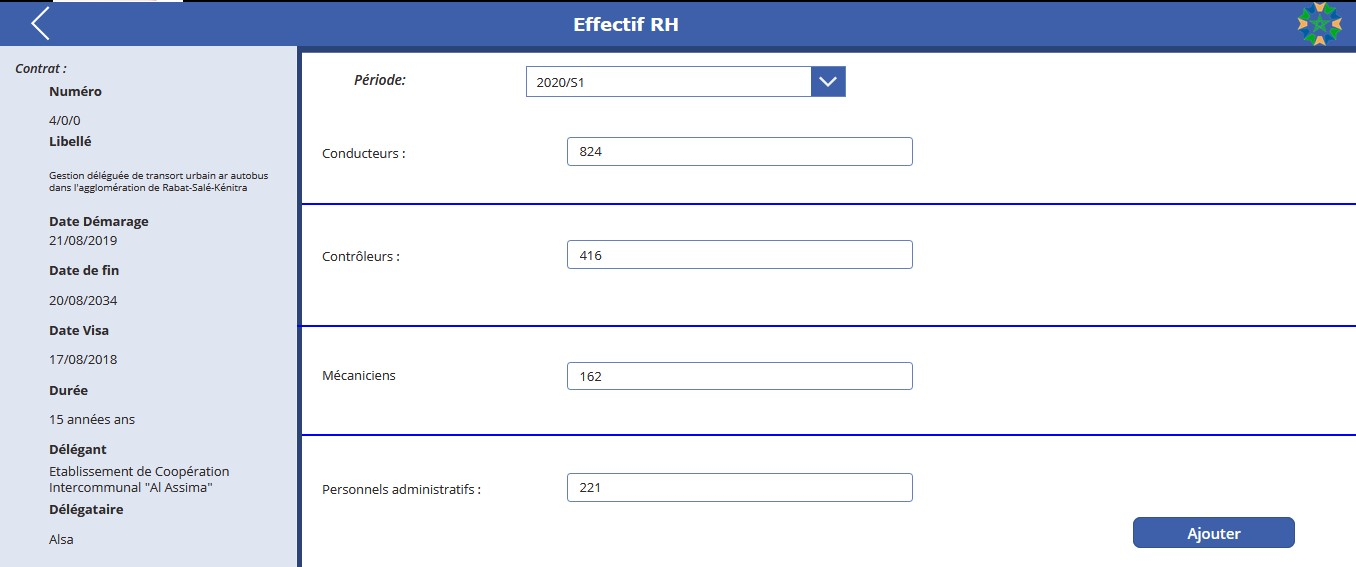
\includegraphics[scale=0.40]{Nv avancement effectif rh.jpg}}
        \caption{Ajouter un avancement}
    \end{center}
\end{figure}
Pour ajouter un avancement, on clique sur le bouton « Ajouter avancement » puis cette page s'affiche qui contient préalablement des données déjà enregistrées selon la période référentiel qu'on a choisi, il suffit de modifier les champs voulus.
\section{Pages Délégants}
\subsection{Liste des délégants}
\begin{figure}[H]
    \begin{center}
        \fbox{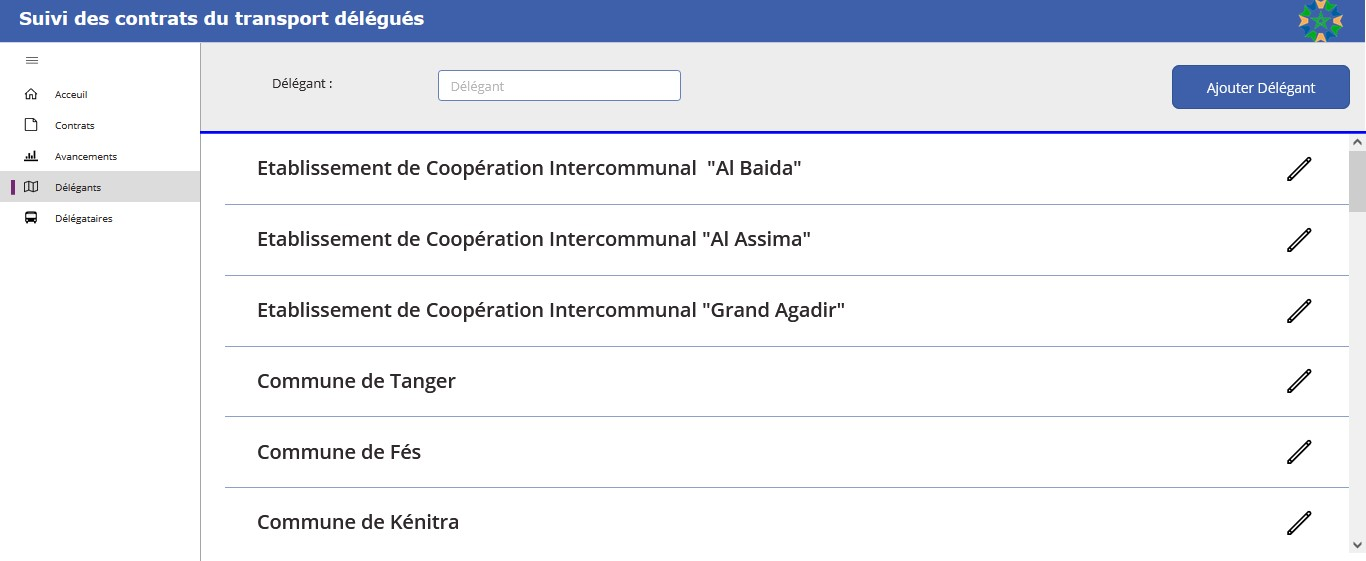
\includegraphics[scale=0.40]{aff delegant.jpg}}
        \caption{Liste des délégants}
    \end{center}
\end{figure}
Cette page nous affiche tous les délégants , comme nous pouvons trouver un délégant rapidement par son nom en le tapant dans la barre de recherche.
\subsection{Modifier un délégant}
\begin{figure}[H]
    \begin{center}
        \fbox{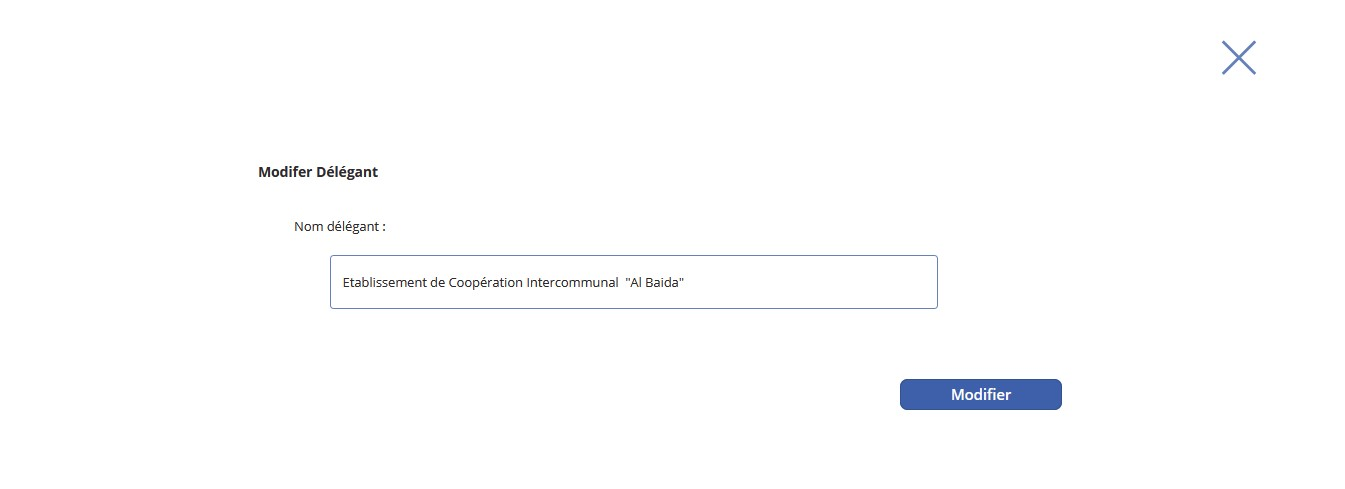
\includegraphics[scale=0.40]{modifier delegant.jpg}}
        \caption{Modifier un délégant}
    \end{center}
\end{figure}
Une fois on clique sur l'icône modifier on se redirige vers cette page pour modifier le nom du délégant.
\subsection{Ajouter un délégant}
\begin{figure}[H]
    \begin{center}
        \fbox{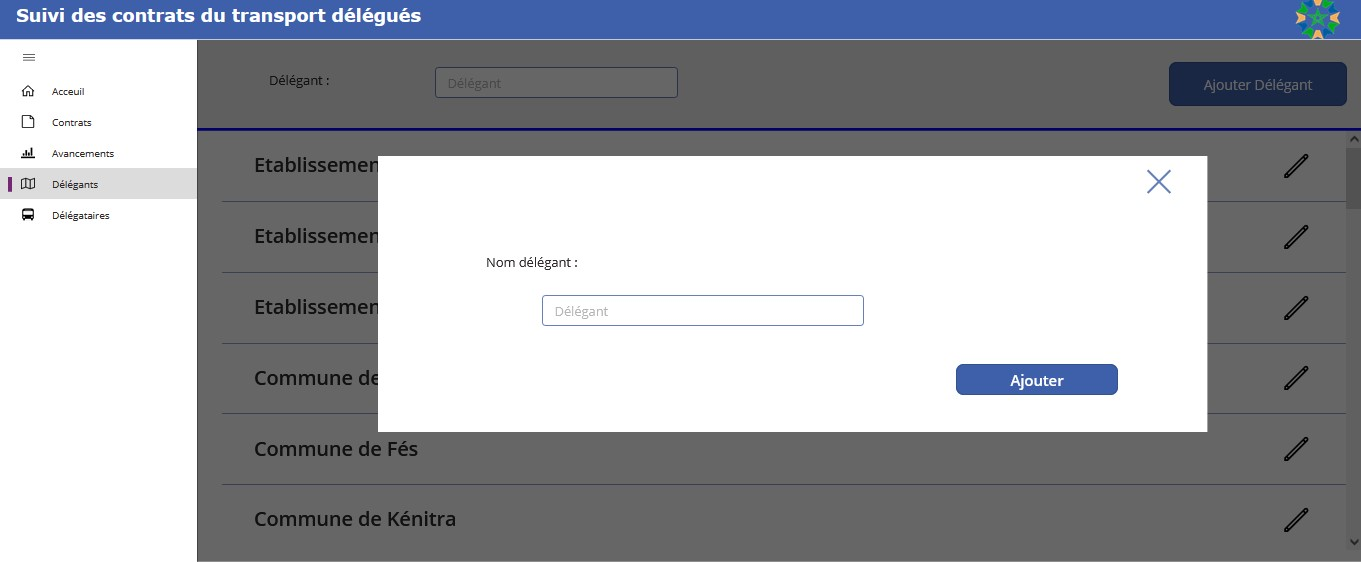
\includegraphics[scale=0.40]{ajouter delegant.jpg}}
        \caption{Ajouter un délégant}
    \end{center}
\end{figure}
Après avoir cliqué sur le bouton « ajouter un délégant » cette pop-up s'affiche, on tape le nom du délégant puis on confirme l'ajout.

\section{Récapitulatif}

Dans ce chapitre, j'ai présenté les interfaces réalisées dans cette application,
Après avoir spécifié et s'adapter avec les outils de travail, j'ai commencé l'implémentation de
l’application et j'ai pu présenter les captures d’écran précédentes.
